\section{Scaling the diffusion world model to \textit{Counter-Strike: Global Offensive}\protect\footnote{This section was added after NeurIPS acceptance, following community interest in later CS:GO experiments.}}
\label{sec:csgo}

To investigate the ability of \textsc{diamond}'s diffusion world model to learn to model more complex 3D environments, we train the world model in isolation on static data from the popular video game \textit{Counter-Strike: Global Offensive} (CS:GO). We use the \textit{Online} dataset of 5.5M frames (95 hours) of online human gameplay captured at 16Hz from the map \textit{Dust II} by \citet{pearce2022counter}. We randomly hold out 0.5M frames (corresponding to 500 episodes, or 8 hours) for testing, and use the remaining 5M frames (87 hours) for training. There is no reinforcement learning agent or online data collection involved in these experiments.

To reduce the computational cost, we reduce the resolution from $(280\times150)$ to $(56\times30)$ for world modeling. We then introduce a second, smaller diffusion model as an upsampler to improve the generated images at the original resolution \citep{saharia2022image}. We scale the channels of the U-Net to increase the number of parameters from 4M for our Atari models to 381M for our CS:GO model (including 51M for the upsampler). The combined model was trained for 12 days on an RTX 4090. 

Finally, we introduce stochastic sampling and increase the number of denoising steps for the upsampler to 10, which we found to improve the resulting visual quality of the generations, while keeping the dynamics model the same (in particular, still using only 3 denoising steps). This enables a reasonable tradeoff between visual quality and inference cost, with the model running at 10Hz on an RTX 3090. Typical generations of the model are provided in Figure \ref{fig:csgo_grid} below.

%%%%%%%%%%%%%%%%%%%%%%%
\begin{figure}[h]
%\vspace{-6mm}
\begin{center}
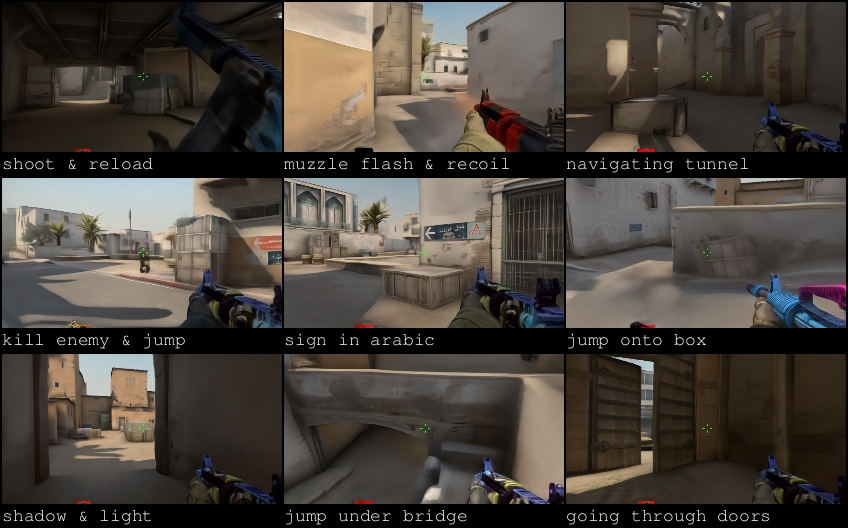
\includegraphics[width=.7\linewidth]{images/csgo_grid.png}
\caption{Images captured from people playing with keyboard and mouse inside \textsc{diamond}'s diffusion world model. This model was trained on $87$ hours of static \textit{Counter-Strike: Global Offensive} (CS:GO) gameplay \citep{pearce2022counter} to produce an interactive neural game engine for the popular in-game map, \textit{Dust II}. Best viewed as videos at \wslink.}
\label{fig:csgo_grid}
\end{center}
\vspace{-4mm}
\end{figure}
%%%%%%%%%%%%%%%%%%%%%%%

We find the model is able to generate stable trajectories over hundreds of timesteps, although is more likely to drift out-of-distribution in less frequently visited areas of the map. Due to the limited memory of the model, approaching walls or losing visibility may cause the model to forget the current state and instead generate a new weapon or area of map. Interestingly, we find the model wrongly enables successive jumps by generalizing the effect of a jump on the geometry of the scene, since multiple jumps do not appear often enough in the training gameplay for the model to learn that mid-air jumps should be ignored. We expect scaling the model and data to address many of these limitations, with the exception of the memory of the model. Quantitative measurements of the capabilities of the CS:GO world model and attempts to address these limitations are left to future work.

% %%%%%%%%%%%%%%%%%%%%%%%
% \begin{wrapfigure}[]{R}{0.55\linewidth}
% \vspace{-5mm}
% \begin{center}
% \centerline{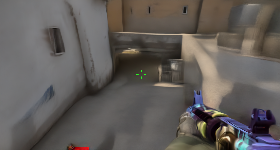
\includegraphics[width=\linewidth]{images/csgo_jump.png}}
% \caption{Looking down at the map after multiple jumps. The model enables multiple jumps by generalizing the effect of a jump on the geometry of the scene, even though only a single jump should be possible. Full video available at \url{https://diamond-wm.github.io}.}
% \label{fig:csgo_jump}
% \end{center}
% \vskip 0in
% \end{wrapfigure}
% %%%%%%%%%%%%%%%%%%%%%%%



% \begin{itemize}
%     \item Motivation: Investigate application of diffusion world model to 3d environment as more complex
%     \item Figure: Example trajectories at different timesteps to show stability (and kb/mouse). Add link to video/website.
%     \item Method: No RL though, things we changed
%     \item Details: In order to reproduce - scaling UNet, discuss actions?, rect not square
%     \item Found stochastic sampling to help
%     \item Results: Playable at 10Hz, long stable trajectories if stay in distribution
%     \item Jump (claim 3d, but be cautious about reasons)
%     \item Limitations + Future work: scaling data/compute, CFG, proper measurements (App J)
% \end{itemize}

% \begin{itemize}
%     \item TODO: Add Generative Game Engine paragraph to related work.
%     \item TODO: update abstract to mention CSGO and website
%     \item TODO: update introduction/conclusion with csgo
%     \item TODO: Update previous CSGO appendix to 'early' experiments
%     \item TODO: Add rebuttal work (training times and DDPM drift) to appendix with mentions from main text
%     \item TODO: Check rebuttal for other promises
% \end{itemize}